\documentclass[12pt]{article}
\usepackage{times} 			% use Times New Roman font

\usepackage[margin=1in]{geometry}   % sets 1 inch margins on all sides
\usepackage[hidelinks]{hyperref}               % for URL formatting
\usepackage[pdftex]{graphicx}       % So includegraphics will work
\setlength{\parskip}{1em}           % skip 1em between paragraphs
\usepackage{indentfirst}            % indent the first line of each paragraph
\usepackage{datetime}
\usepackage[small, bf]{caption}
\usepackage{listings}               % for code listings
\usepackage{xcolor}                 % for styling code
\usepackage{multirow}
\usepackage{adjustbox}
\usepackage{caption}


%New colors defined below
\definecolor{backcolour}{RGB}{246, 246, 246}   % 0xF6, 0xF6, 0xF6
\definecolor{codegreen}{RGB}{16, 124, 2}       % 0x10, 0x7C, 0x02
\definecolor{codepurple}{RGB}{170, 0, 217}     % 0xAA, 0x00, 0xD9
\definecolor{codered}{RGB}{154, 0, 18}         % 0x9A, 0x00, 0x12

%Code listing style named "gcolabstyle" - matches Google Colab
\lstdefinestyle{gcolabstyle}{
  basicstyle=\ttfamily\small,
  backgroundcolor=\color{backcolour},   
  commentstyle=\itshape\color{codegreen},
  keywordstyle=\color{codepurple},
  stringstyle=\color{codered},
  numberstyle=\ttfamily\footnotesize\color{darkgray}, 
  breakatwhitespace=false,         
  breaklines=true,                 
  captionpos=b,                    
  keepspaces=true,                 
  numbers=left,                    
  numbersep=5pt,                  
  showspaces=false,                
  showstringspaces=false,
  showtabs=false,                  
  tabsize=2
}

\lstset{style=gcolabstyle}      %set gcolabstyle code listing

% to make long URIs break nicely
\makeatletter
\g@addto@macro{\UrlBreaks}{\UrlOrds}
\makeatother

% for fancy page headings
\usepackage{fancyhdr}
\setlength{\headheight}{13.6pt} % to remove fancyhdr warning
\pagestyle{fancy}
\fancyhf{}
\rhead{\small \thepage}
\lhead{\small HW\#4, Huang}  % EDIT THIS, REPLACE # with HW number
\chead{\small DATA 440, Fall 2022} 

%-------------------------------------------------------------------------
\begin{document}

% EDIT THE ITEMS HERE
\begin{centering}
{\large\textbf{Exploring Social Networks}}\\ 
Sofia Huang\\
due 11/03/2022\\
\end{centering}

%-------------------------------------------------------------------------

% The * after \section just says to not number the sections
\section*{1. Friendship Paradox on Facebook}
\noindent \textbf{Determine if the friendship paradox holds for a user's Facebook account. (This used to be more interesting when you could more easily download your friend's friends list from Facebook. Facebook now requires each friend to approve this operation, effectively making it impossible.)\\
\\acnwala\_friends\_friends\_count.csv (provided on Piazza) contains a user's friends' names and number of friends they each have.\\
\\Create a graph of the number of friends (y-axis) and the friends themselves (x-axis), sorted by number of friends. The friends don't need to be labeled on the x-axis: 1, 2, 3,..., n should be sufficient. Include the user in the graph in the appropriate sorted position (count the number of their friends) and label as U.}

I used the .csv file given by Prof. Nwala and imported it as a DataFrame. Then, I sorted the values based on friend count and added Prof. Nwala and his own friendcount into the DataFrame at the correct position. I used Matplotlib to plot the bar graph to show the data and to prove the friendship paradox holds.

\begin{lstlisting}[language=python, caption=plotting Prof. Nwala's Facebook friends' friend count, label=lst:copy]
def plot_friends(df, filename):
    # sort df values and reset index
    df = df.sort_values('FRIENDCOUNT')
    df = df.reset_index(drop=True)
    index = np.arange(1,99)
    df['INDEX'] = index
    # add Prof. Nwala's data to the df
    df2 = {'USER': 'Alexander Nwala', 'FRIENDCOUNT': 98, 'INDEX': 'U'}
    line = pd.DataFrame(df2, index=[10])
    df2 = pd.concat([df.iloc[:10], line, df.iloc[10:]]).reset_index(drop=True)
    # plot the bar graph and fix details
    plt.figure(figsize=(36, 8))

    ax = plt.gca()
    ax.margins(x=0)

    plt.bar(df2.index, df2['FRIENDCOUNT'], width=0.6)
    plt.xticks(np.arange(len(df2['INDEX'])), df2['INDEX'],fontsize='18')
    plt.xlabel('Users', fontsize=24)
    plt.ylabel('Friend Count', fontsize=24)
    plt.title('Friendship Paradox', fontsize=30)
    # save plot to file

    plt.tight_layout()
    plt.savefig(filename)
    #plt.show()
\end{lstlisting}

\noindent\textbf{Q: What is the mean, standard deviation, and median of the number of friends that the user's friends have?}

\begin{lstlisting}[language=bash, caption=summary statistics for Facebook friends, label=lst:copy]
The mean of the number of friends that the user`s friends have: 542.6734693877551
The median of the number of friends that the user`s friends have: 396.0
The standard deviation of the number of friends that the user`s friends have: 536.6744685696292
\end{lstlisting}

\begin{figure}[h]
    \centering
    % trim and clip are used to crop the image, trim=left bottom right top
    % width sets max width, height will be scaled appropriately
    %\includegraphics[trim=0 20 10 50, clip, width=\textwidth]
    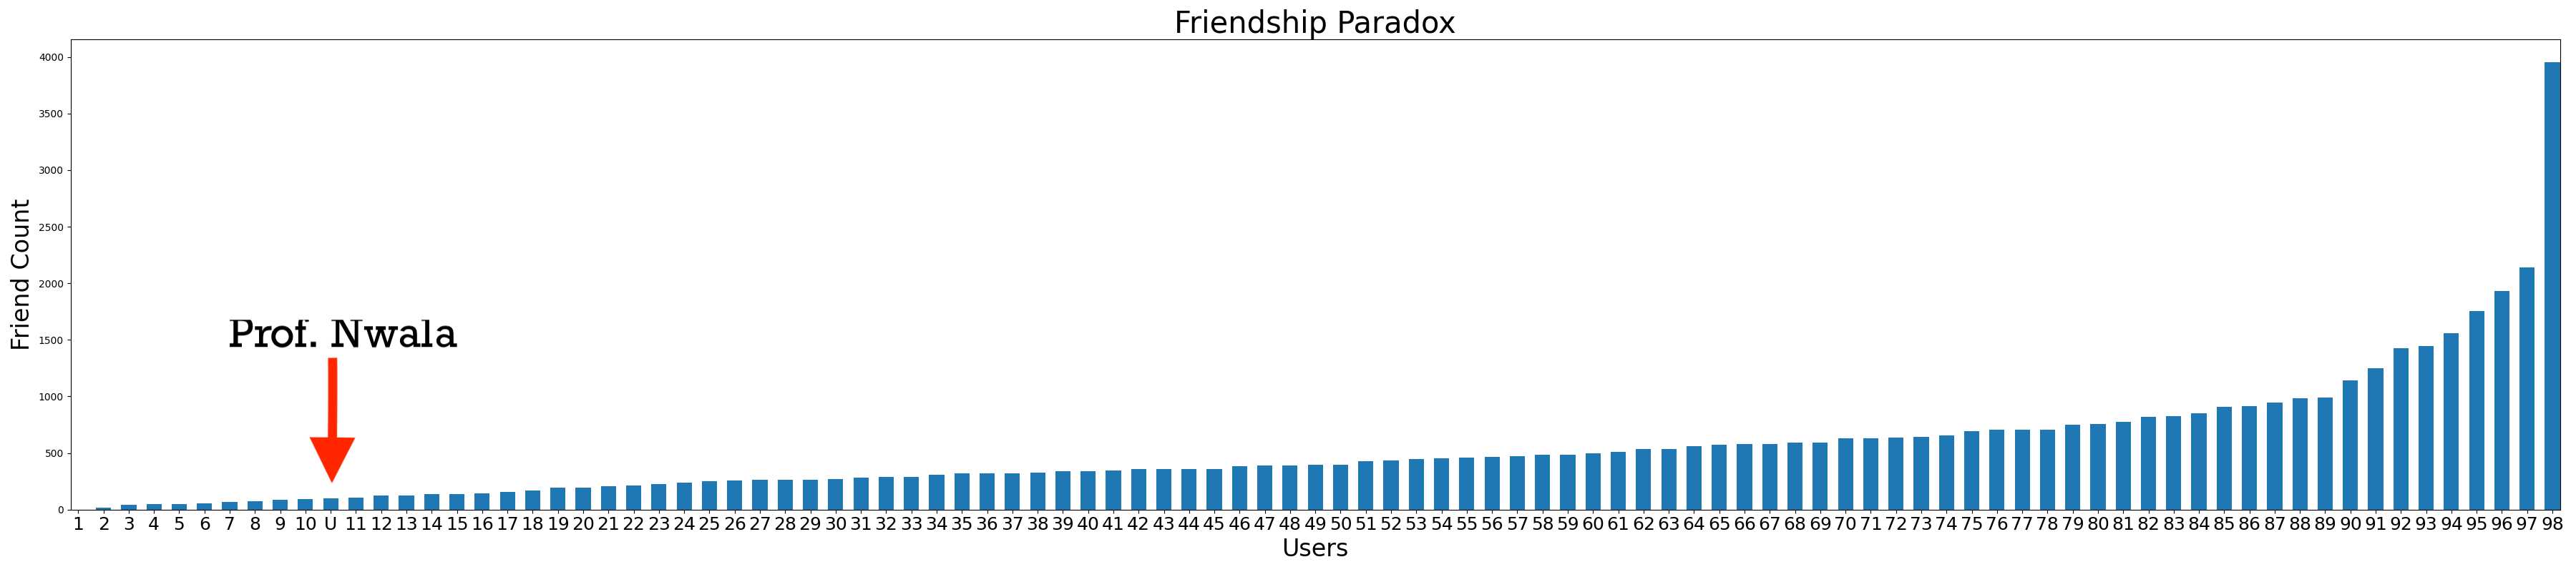
\includegraphics[width=\textwidth, scale=1.5]
    {friendship_paradox_barplot2.png}
    \caption{Friend count of Prof. Nwala and his friends on Facebook, sorted by friend count.}
    \label{fig:friendship-paradox}
\end{figure}

\noindent\textbf{Q: Does the friendship paradox hold for this user and their friends on Facebook?}

The friendship paradox does hold for this user and their friends on Facebook because the average of the user's friends' friends is 876, while the user only has 98 friends on Facebook. So, on average, the user's friends, have more friends than the user themselves.

\section*{2. Friendship Paradox on Twitter}
\noindent \textbf{Determine if the friendship paradox holds for your Twitter account. Since Twitter is a directed graph, use followers as the value you measure (i.e., "do your followers have more followers than you?").}

I used twarc to get a list of my own followers as a .jsonl file. Using this file, I was able to obtain their follower counts by parsing the data structure returned from Twitter. I used a dictionary to store the follower's username and their follower count. Then, I converted the dictionary to a .csv file to save it to my computer.

\begin{lstlisting}[language=bash, caption=obtaining my own followers using twarc, label=lst:copy]
twarc2 followers _sofiahuang myfollowers.jsonl
\end{lstlisting}

\begin{lstlisting}[language=python, caption=obtaining my followers' follower count, label=lst:copy]
def get_followers_followers(jsonl_file):
    f = open(jsonl_file)
    # read in all the lines
    lines = f.readlines()  
    followers_stats = {}
    # add a header entry to dictionary for the csv later
    followers_stats.update({'USER':'FRIENDCOUNT'})
    # each line is a json 
    for line in lines:
        follower_data = json.loads(line)
        # get my follower count
        num_my_followers = follower_data['meta']['result_count']
        print(num_my_followers)
        # loop through my followers and get their username + follower count
        # to add to a dictionary
        for i in range(num_my_followers):
            follower_username = follower_data['data'][i]['username']
            follower_followers =  follower_data['data'][i]['public_metrics']['followers_count']
            print('username: {} \nfollower_count: {}'.format(follower_username, follower_followers))
            followers_stats.update({follower_username:follower_followers})
    # add myself to the dictionary
    followers_stats.update({'_sofiahuang':num_my_followers})

    # open file for writing dictionary to csv file
    w = csv.writer(open("/Users/sofiahuang/Documents/WM/FALL2022/DATA440/followers_followers.csv", "w"))
    # loop over dictionary keys and values
    for key, val in followers_stats.items():
        # write every key and value to file
        w.writerow([key, val])
\end{lstlisting}

\noindent\textbf{Q: What is the mean, standard deviation, and median of the number of followers that your followers have?}

\begin{lstlisting}[language=bash, caption=summary statistics for Twitter followers, label=lst:copy]
The mean of the number of friends that my friends have on Twitter: 876.3305084745763
The median of the number of friends that my friends have on Twitter: 175.0
The standard deviation of the number of friends that my friends have on Twitter: 5092.913779325692
\end{lstlisting}


\noindent\textbf{Q: Does the friendship paradox hold for you and your followers on Twitter?}

The friendship paradox holds for me and my friends on Facebook. The average of my followers' number of followers is 876. This number is skewed due to an outlier that has over 30k followers, but even the median of my followers' follower count is 175, compared to my own follower count of 117. So, my followers have more followers than me, on average.

\section*{References}

\begin{itemize}
    \item{Twarc - Getting followers for a list of usernames} \url{https://twittercommunity.com/t/twarc2-getting-followers-for-a-list-of-usernames/176959/2}
\end{itemize}

\end{document}





